\documentclass[12pt]{article}
\usepackage[margin=2cm]{geometry} 
\usepackage{titling}
\usepackage{graphicx}
\usepackage{float}
\usepackage[hidelinks]{hyperref}
\usepackage[italian]{babel}
\usepackage{subcaption}

\setlength\parindent{0pt}
\setlength{\parskip}{1em}
\setlength{\droptitle}{-2cm}

\title{Istruzioni d'uso WarpMe (ad uso interno)}
\author{Università della Svizzera Italiana}
\date{Versione \today}


\begin{document}
\maketitle
\tableofcontents
\newpage


\section{Installazione}\label{installation}	

	\subsection{Componenti}
	
		Il sistema WarpMe è composto dai seguenti elementi:
		
		- schermo tattile
		
		- supporto per schermo tattile
		
		- mini computer Intel NUC
		
		- webcam Logitech HD Pro C920
		
		- stampante Canon Selphy CP1200\\
		
		e dai seguenti cavi:
		
		- 1 cavo HDMI
		
		- 1 cavo tre poli per alimentazione schermo
		
		- 1 adattatore corrente per NUC
		
		- 1 cavo USB-B per schermo tattile
		
		- 1 cavo miniUSB per stampante
		
		- 1 adattatore corrente per stampante
		
		
	\subsection{Montaggio}
	
		\textbf{ATTENZIONE}: per motivi di sicurezza, procedere con la manipolazione dello schermo solo ed esclusivamente in due o più persone.
		
		Appoggiare lo schermo sull'apposito supporto, in verticale, verificando che entrambi i ganci siano fermamente appoggiati al supporto (vedi foto sottostanti). Dopodiché collocare la webcam sul lato destro con l'apposito velcro, fissare il NUC sull'apposito supporto a retro dello schermo e disporre la stampante in un luogo facilmente accessibile (per esempio su un tavolo o piedistallo a lato). Collocare i due alimentatori di NUC e stampante sul piano inferiore del piedistallo.
		
		Aprire il pannello anteriore della stampante e collocare il vassoio portacarta. Controllare il display della stampante e se necessario inserire o sostituire la cartuccia aprendo l'apposito sportello sul lato destro della stampante.
		
	\begin{figure}[H]
		\begin{subfigure}{0.5\textwidth}
                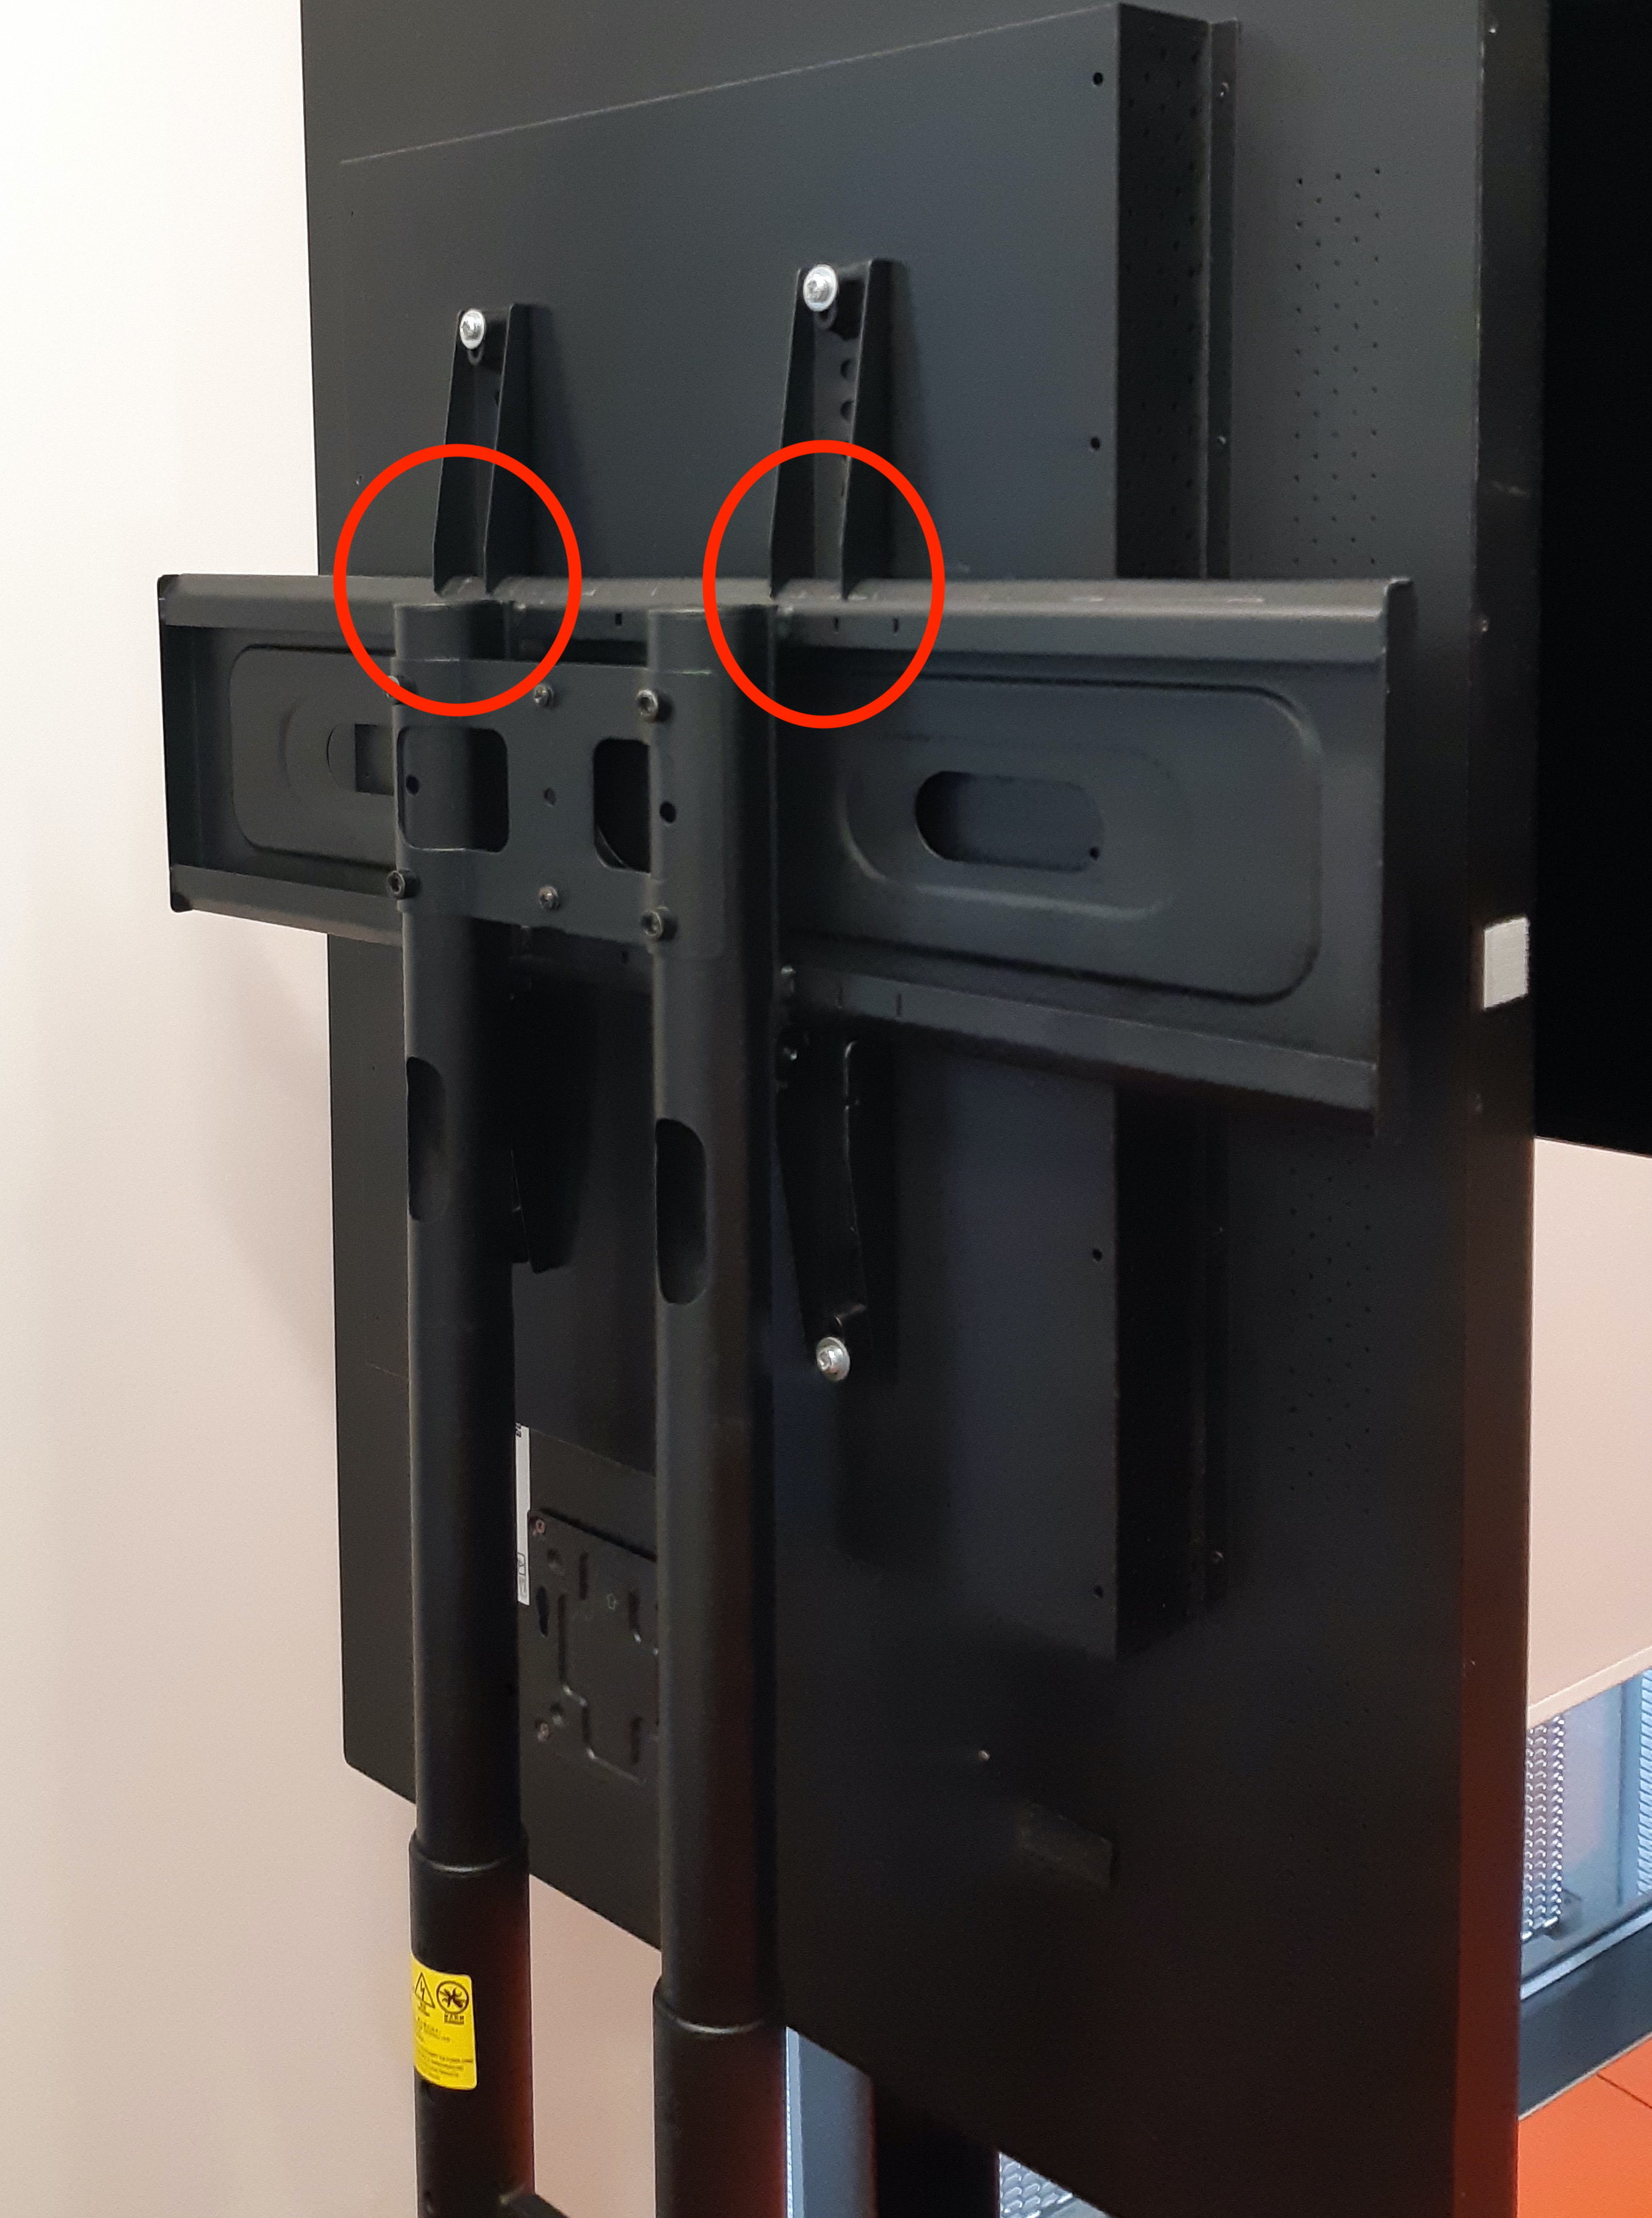
\includegraphics[width=0.9\textwidth]{img/stand_1.jpg}
                \caption*{Lo schermo agganciato}
        \end{subfigure}
		\begin{subfigure}{0.5\textwidth}
                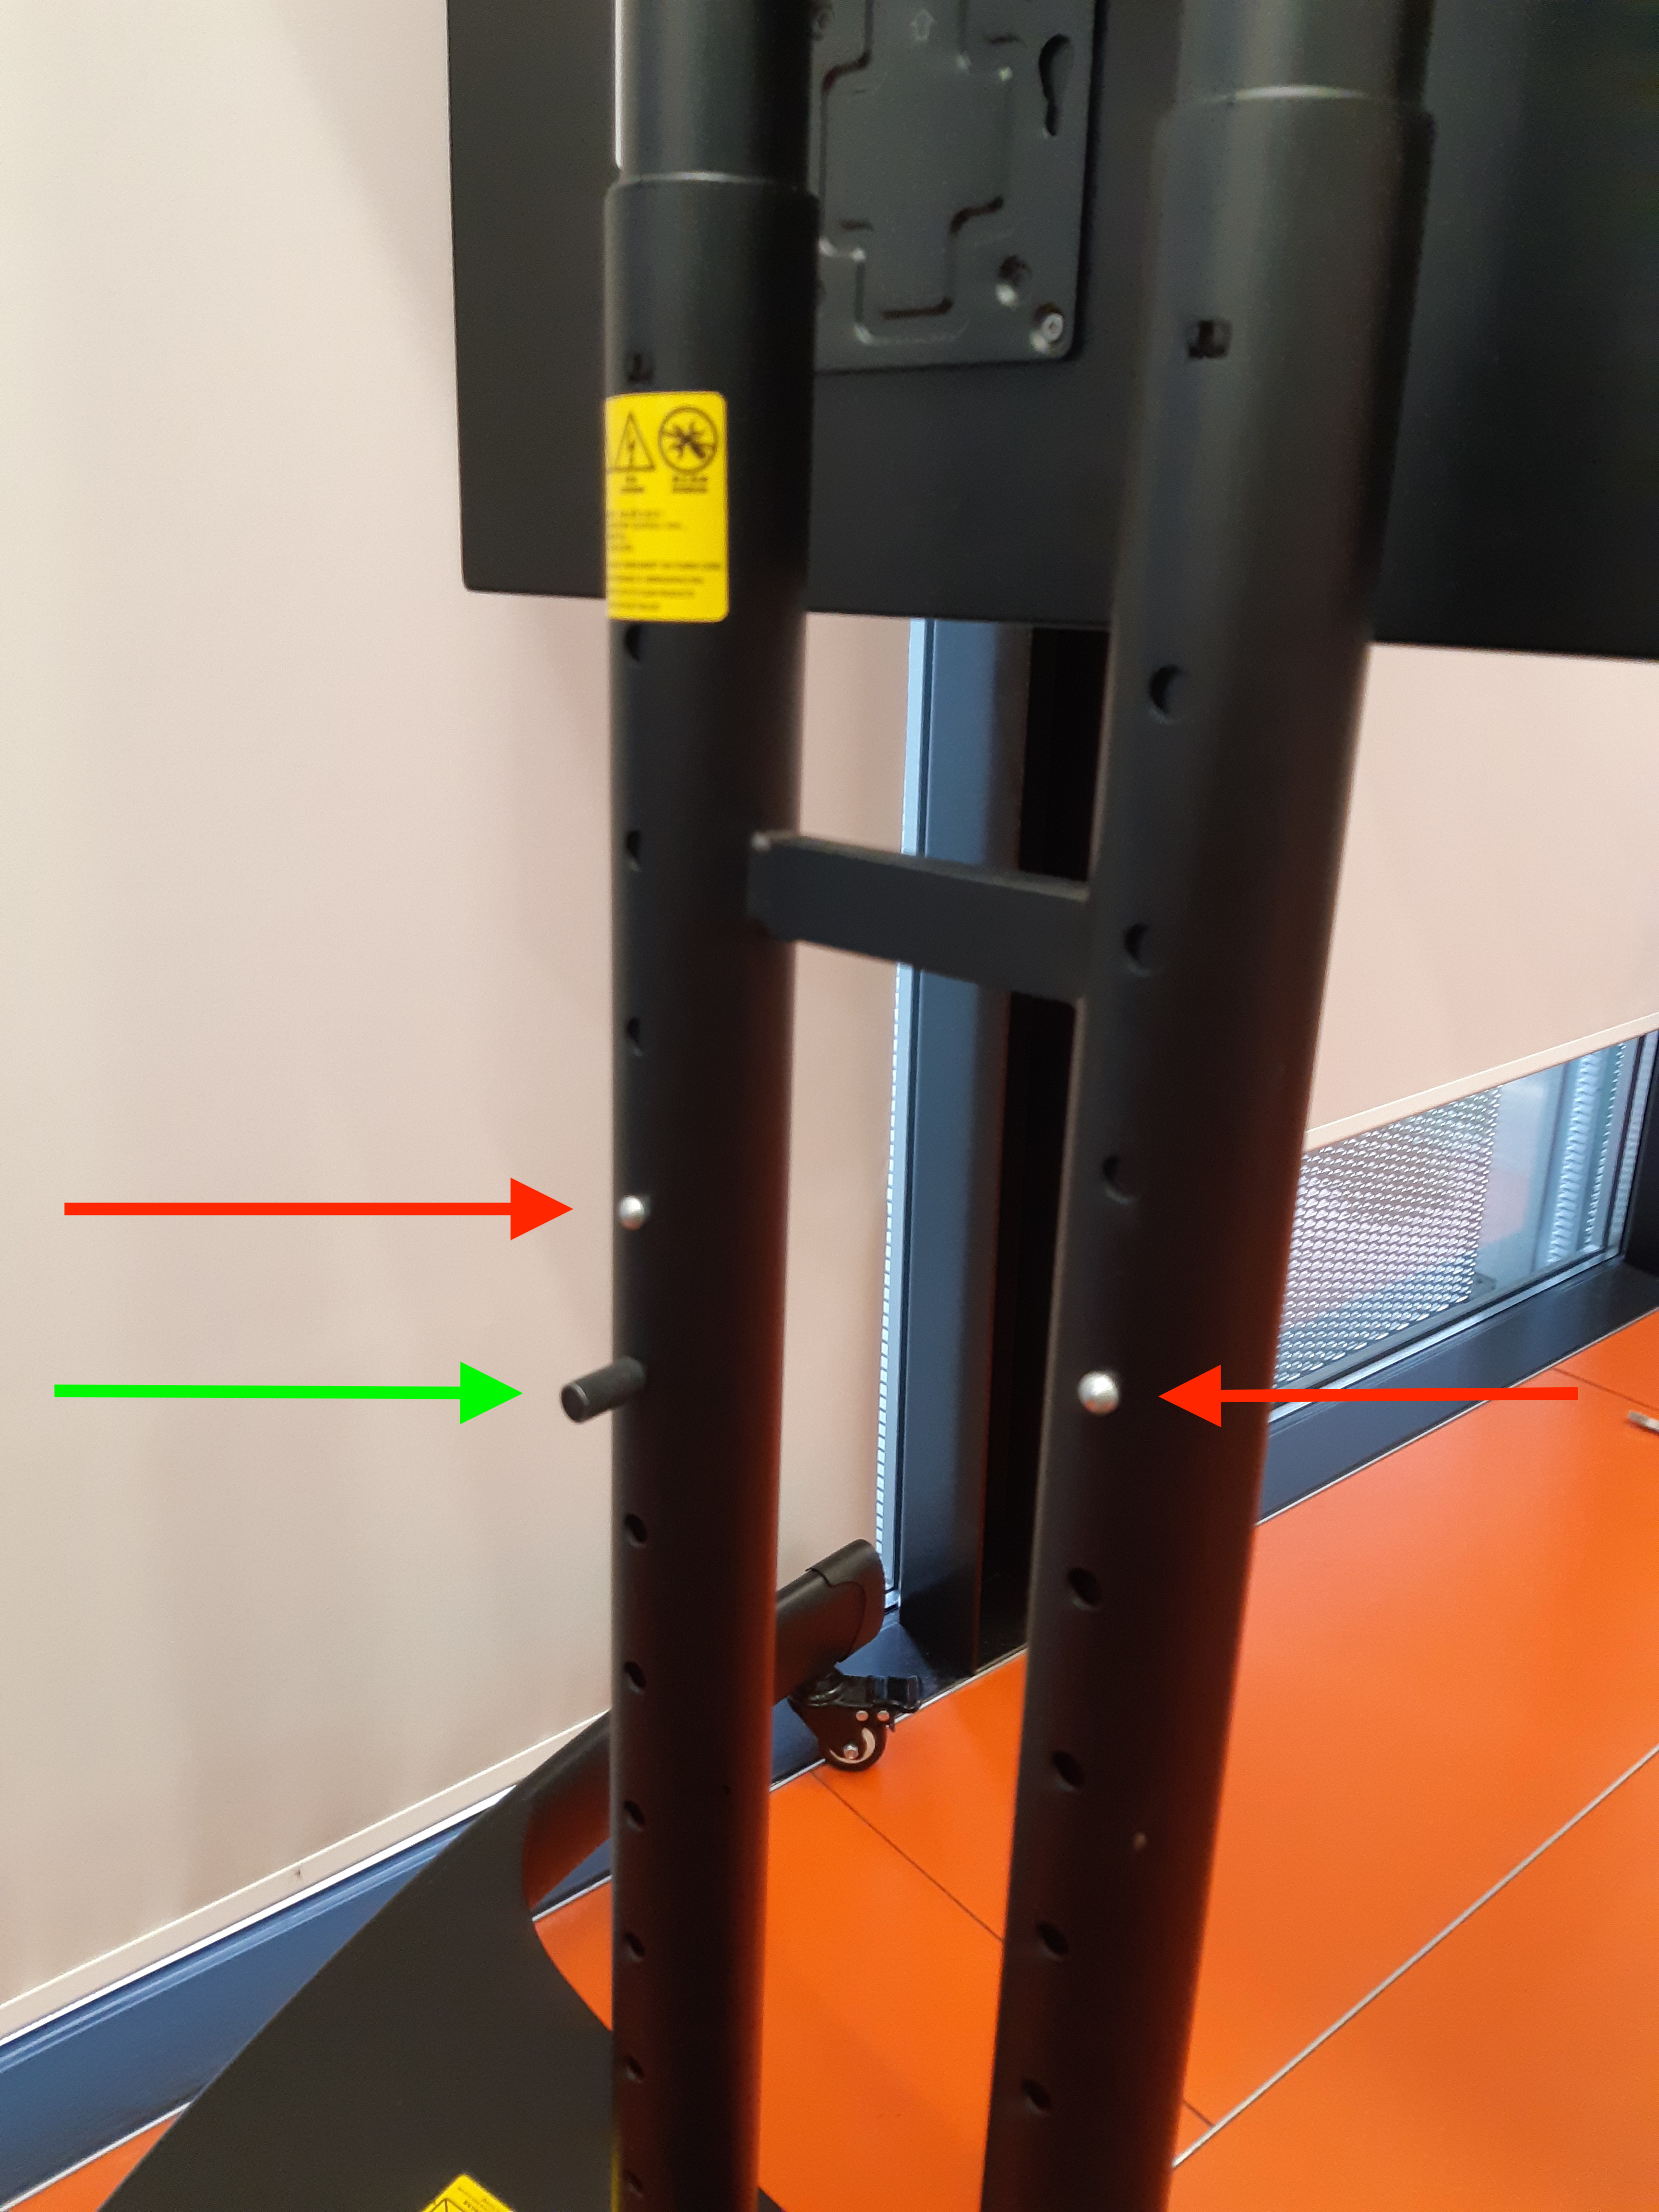
\includegraphics[width=0.9\textwidth]{img/stand_2.jpg}
                \caption*{Regolazione dell'altezza}
        \end{subfigure}
    \end{figure}
    
    \begin{figure}[H]
		\begin{subfigure}{0.5\textwidth}
                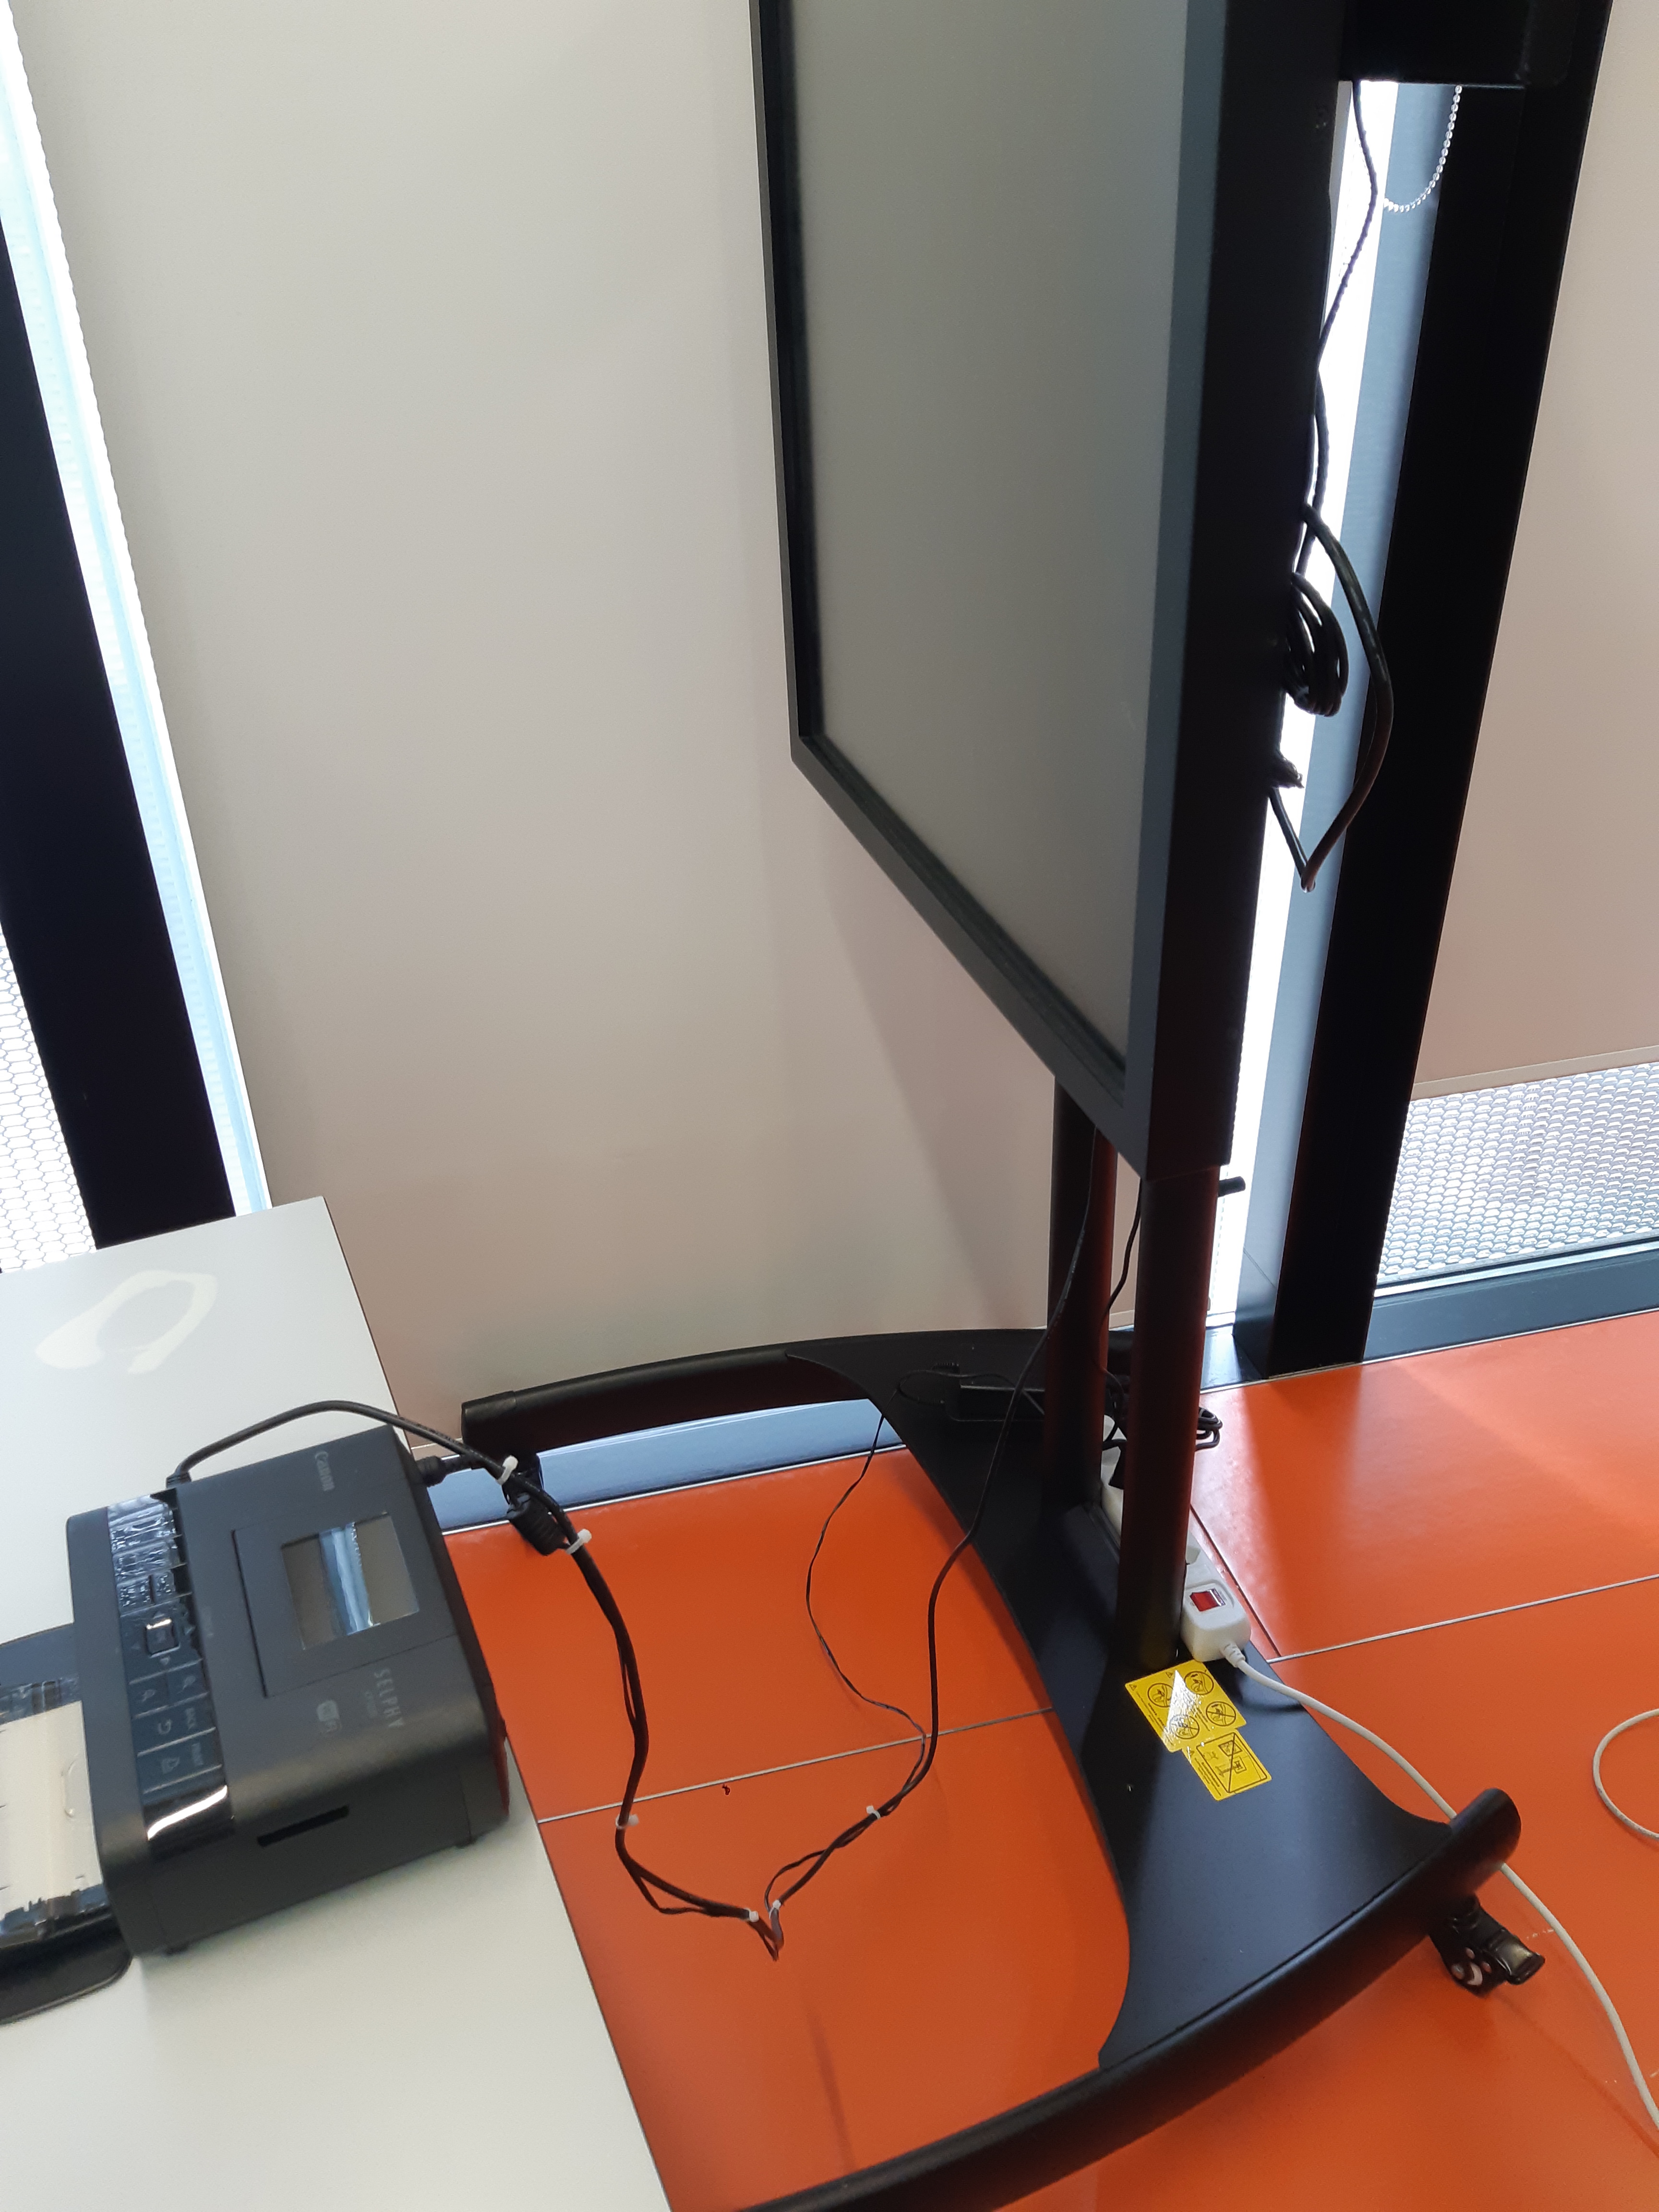
\includegraphics[width=0.9\textwidth]{img/stand_full.jpg}
                \caption*{Il sistema dal fronte}
        \end{subfigure}
		\begin{subfigure}{0.5\textwidth}
                \includegraphics[width=0.9\textwidth]{img/cables_behind.jpg}
                \caption*{Il sistema dal retro}
        \end{subfigure}
    \end{figure}
		
	\begin{figure}[H]
		\begin{subfigure}{0.5\textwidth}
                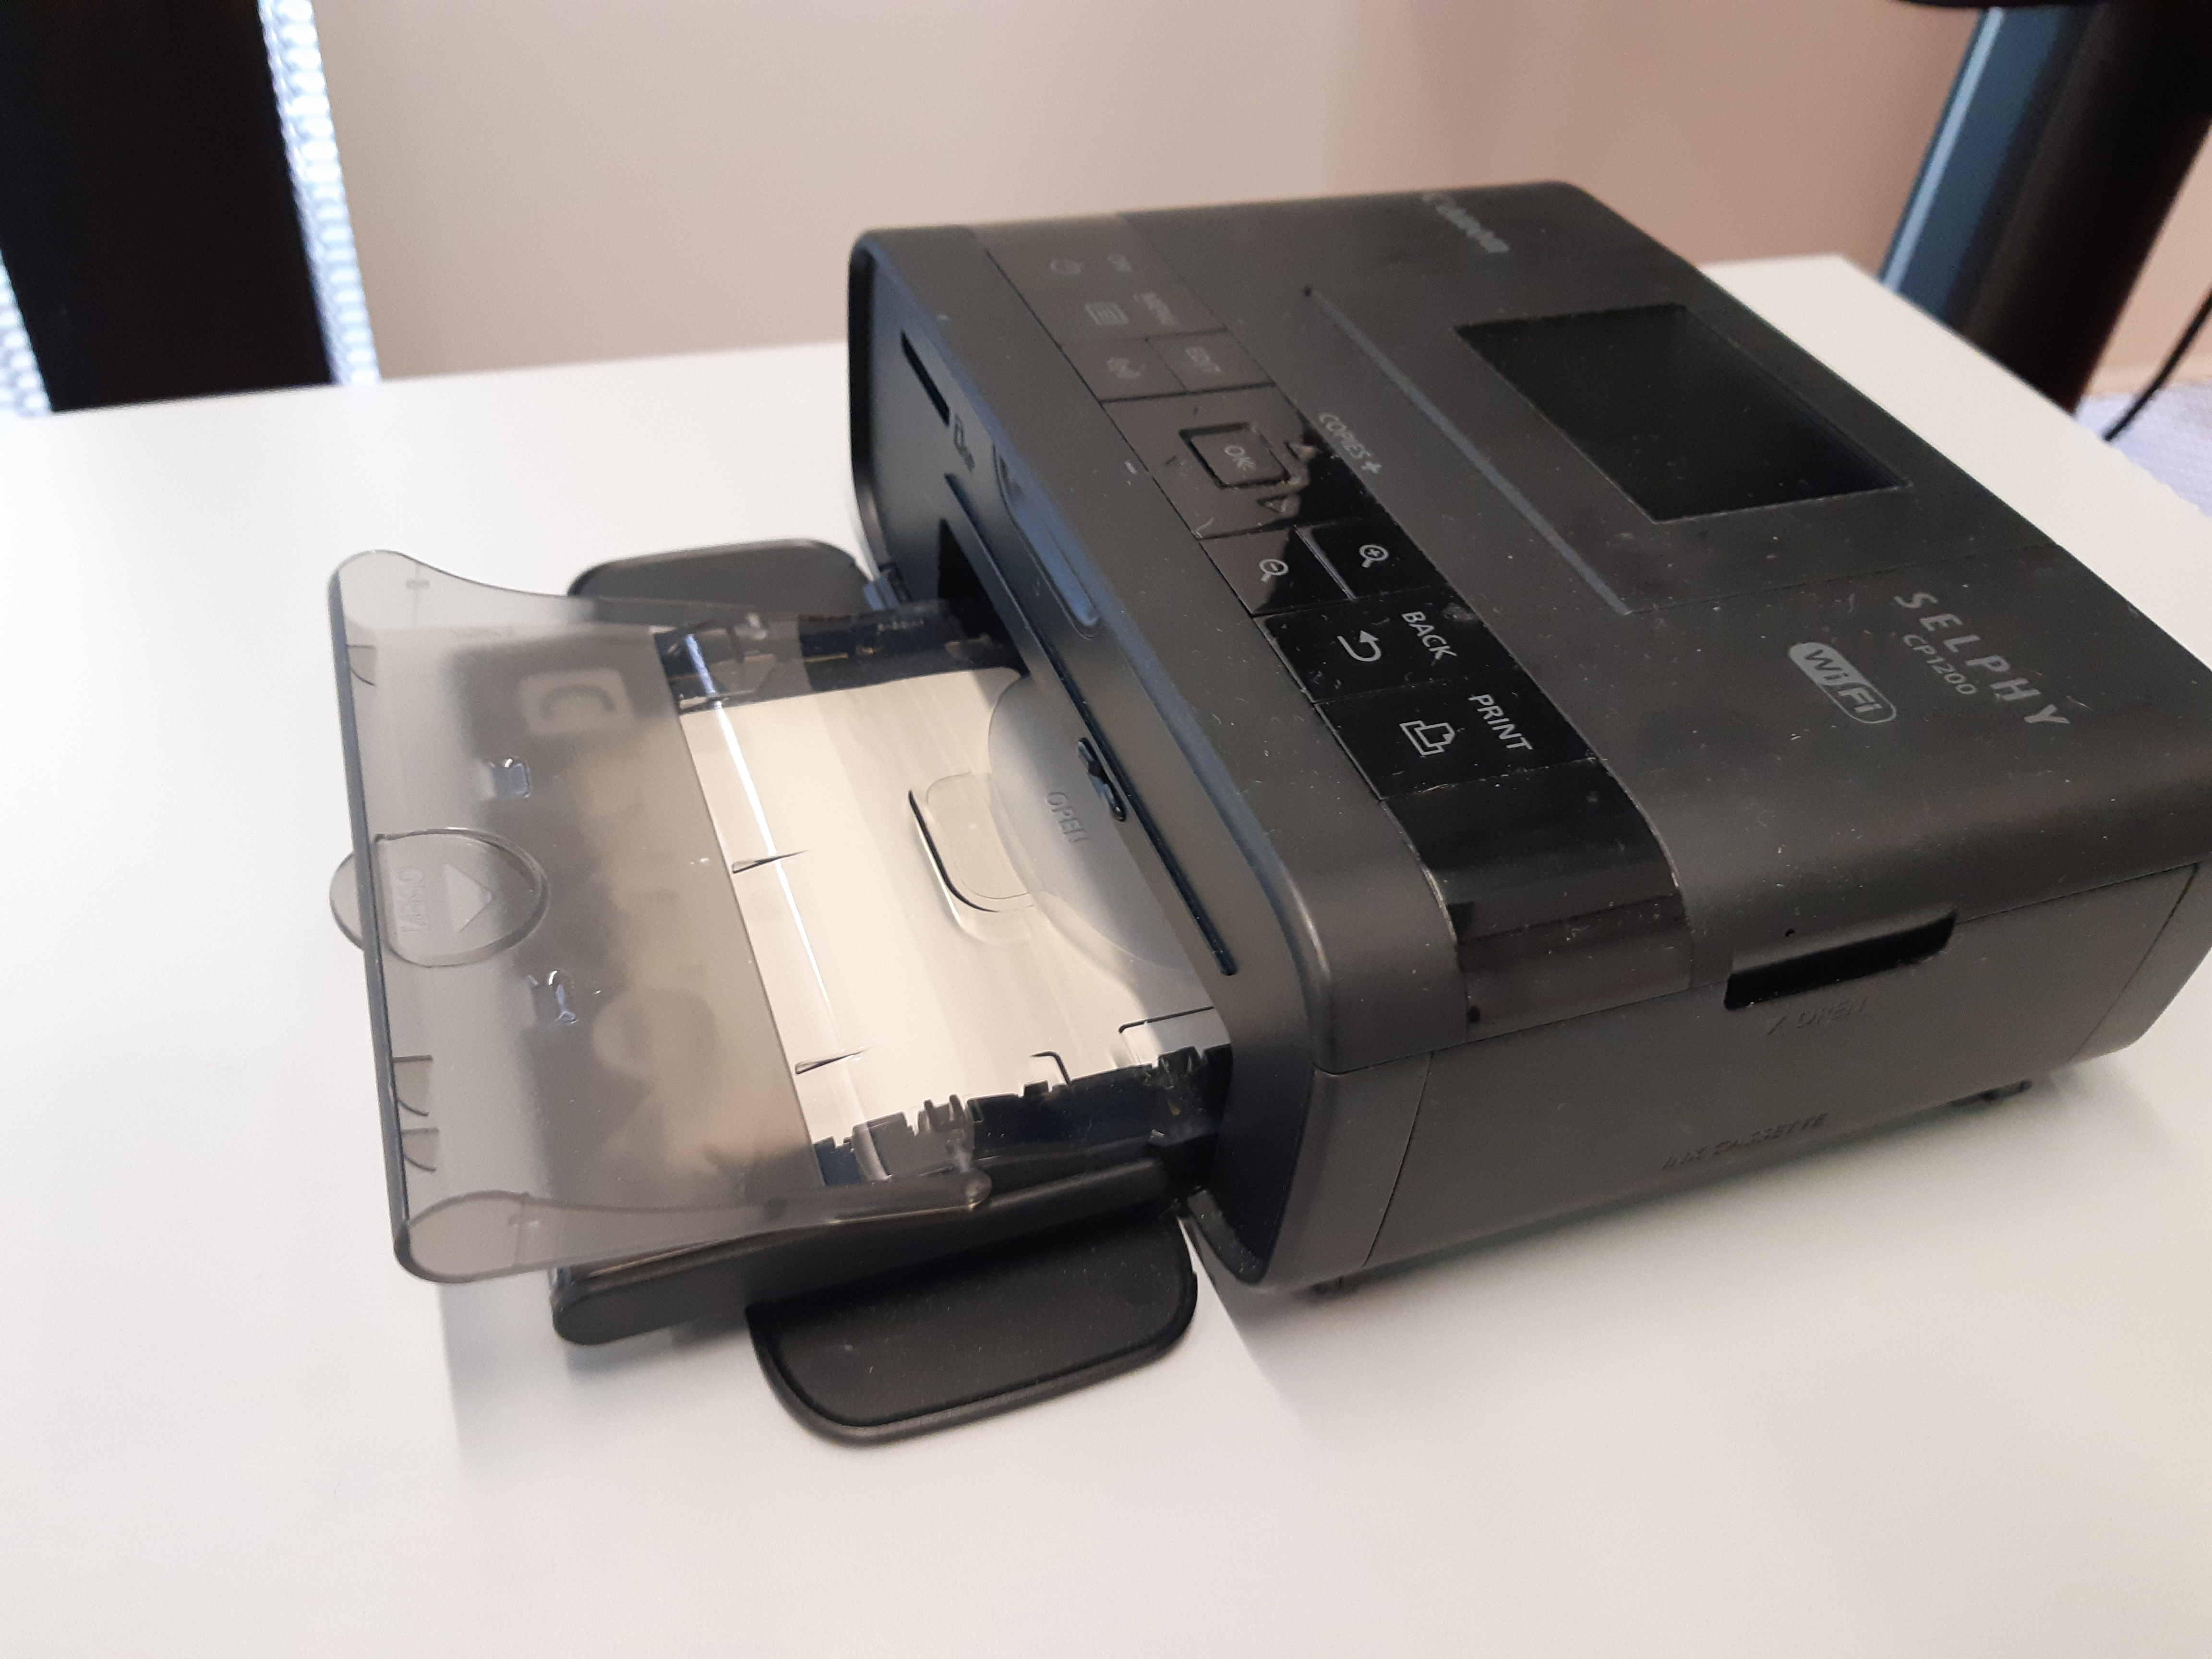
\includegraphics[width=0.9\textwidth]{img/printer.jpg}
                \caption*{La stampante assemblata}
		\end{subfigure}		
		\begin{subfigure}{0.5\textwidth}
                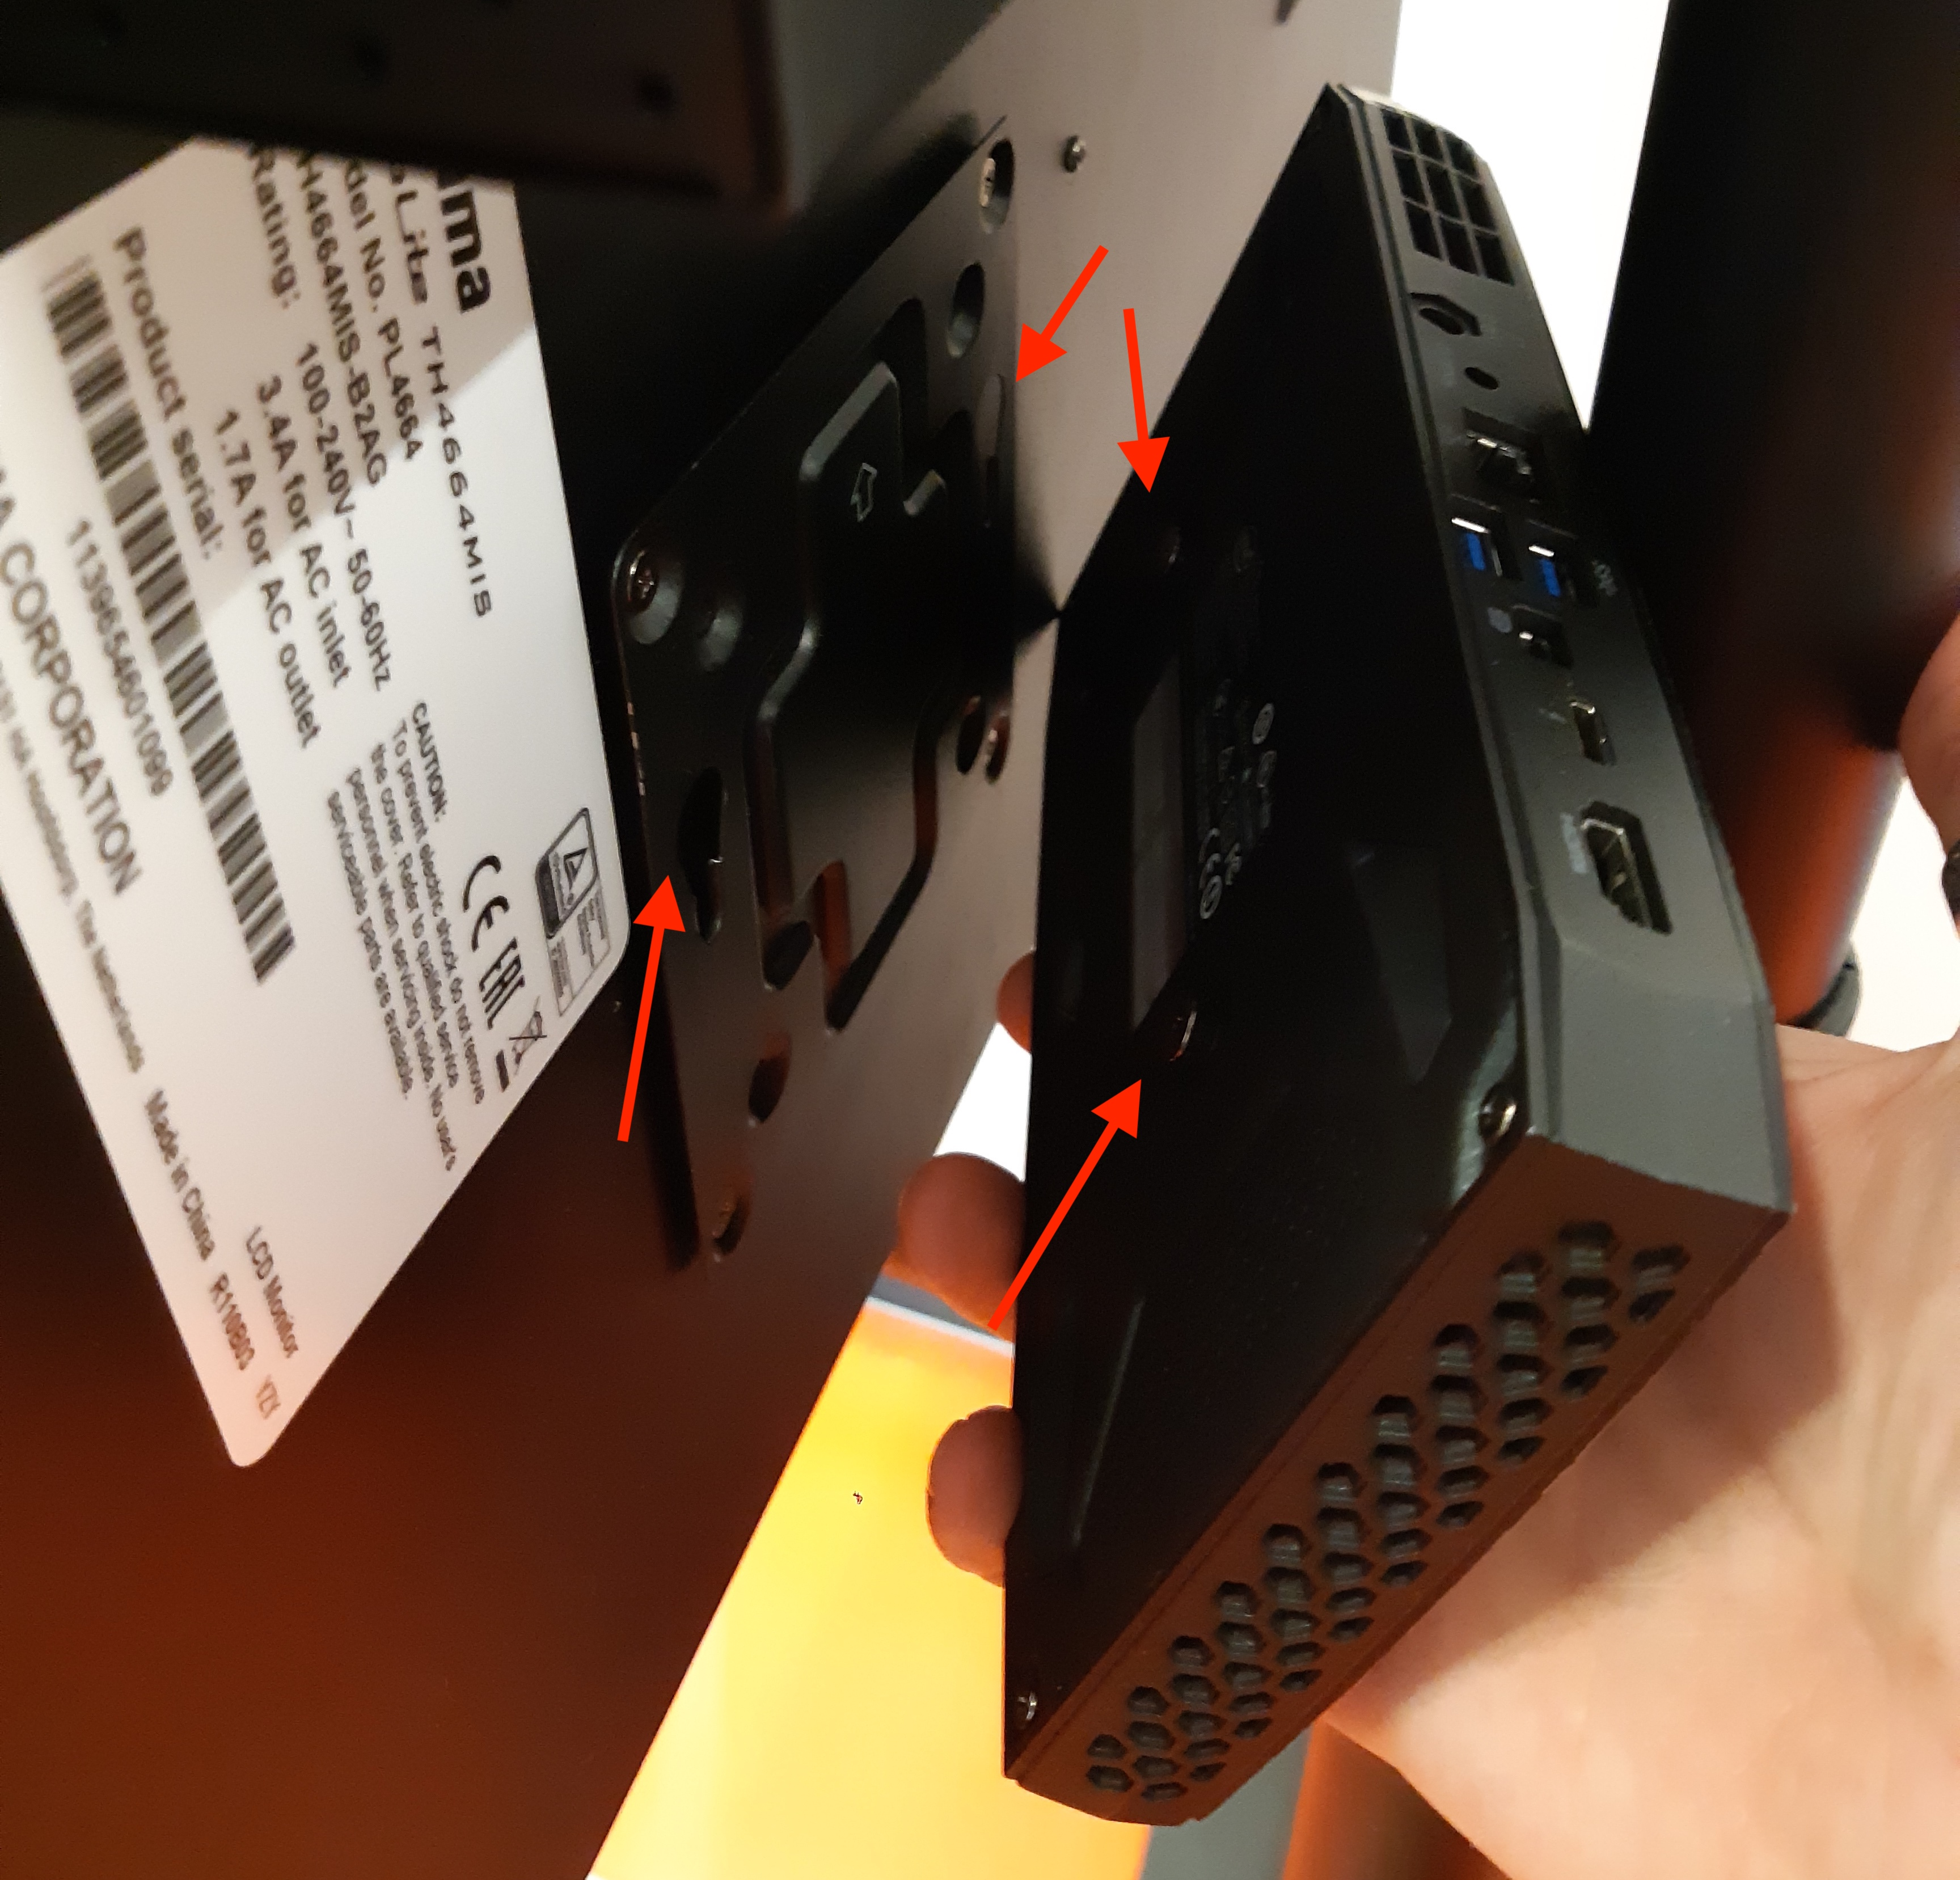
\includegraphics[width=0.9\textwidth]{img/nuc_1.jpg}
                \caption*{Montaggio del NUC}
        \end{subfigure}
    \end{figure}
        
    \begin{figure}[H]
        \begin{subfigure}{0.5\textwidth}
                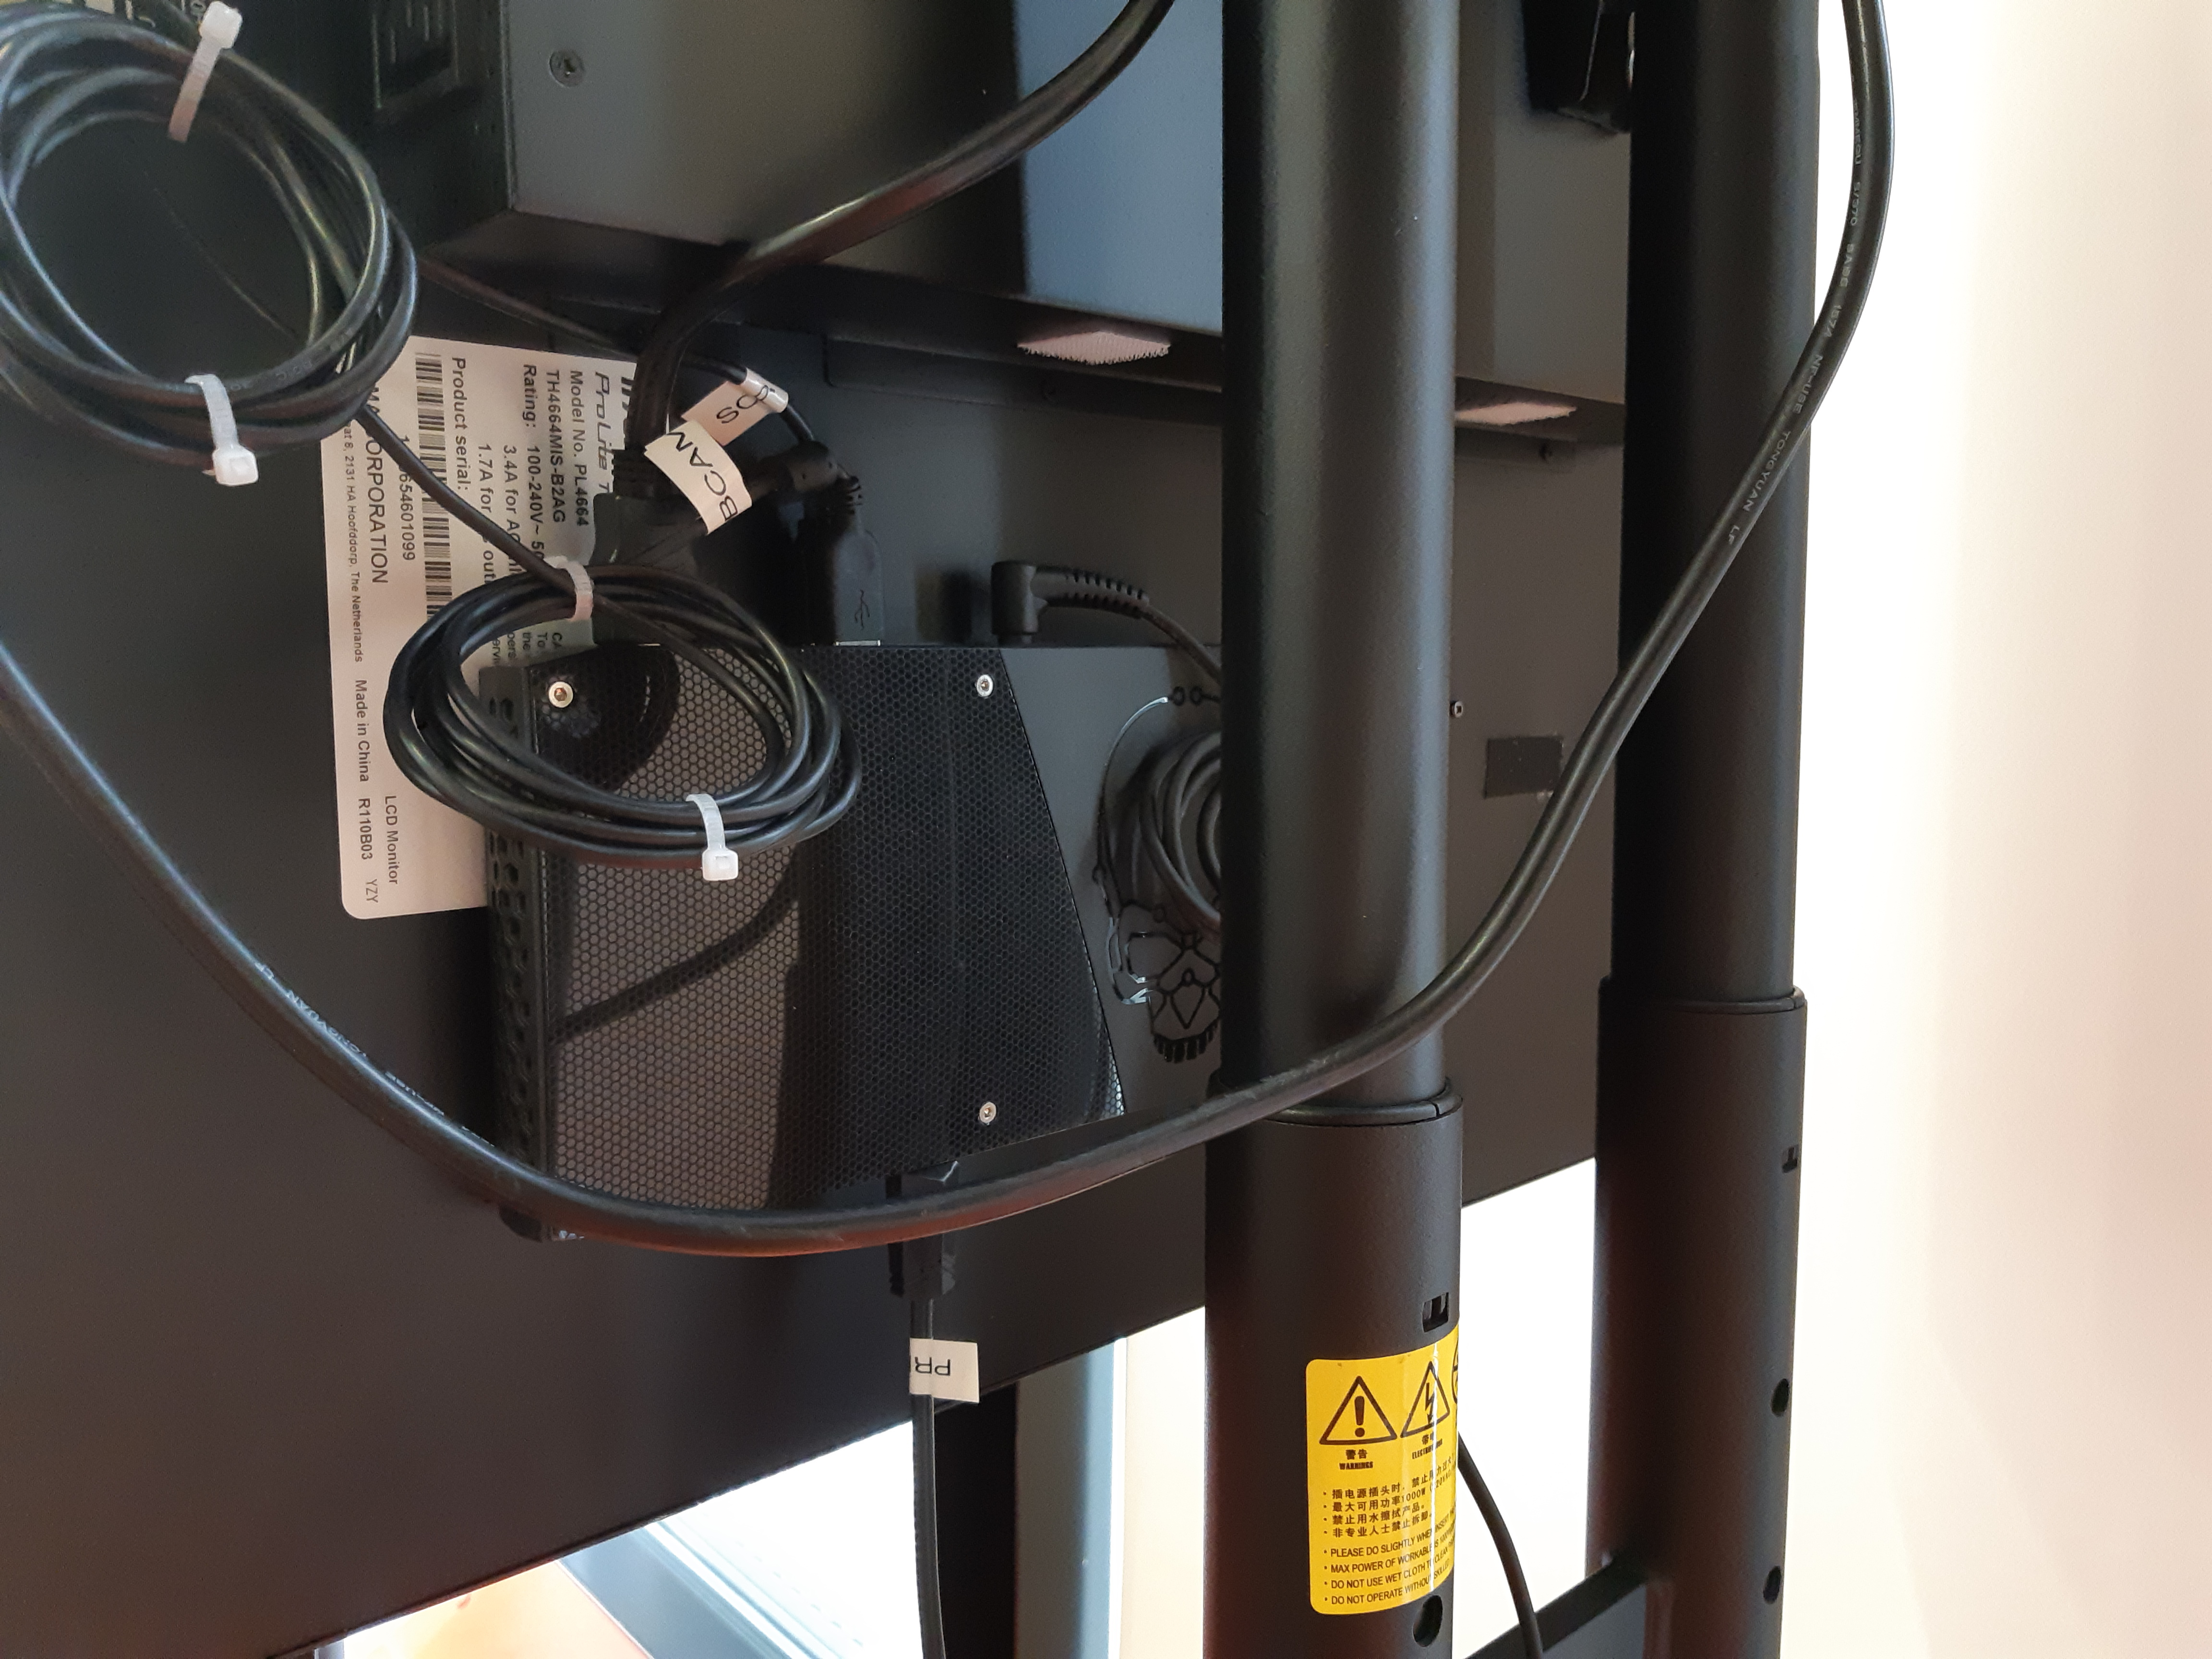
\includegraphics[width=0.9\textwidth]{img/nuc_2.jpg}
                \caption*{Il NUC in posizione}
        \end{subfigure}        
        \begin{subfigure}{0.5\textwidth}
                \includegraphics[width=0.9\textwidth]{img/cables_bottom.jpg}
                \caption*{Alimentazione del sistema}
		\end{subfigure}                
	\end{figure}	
    
    \newpage
    
    
	\subsection{Collegamento}
	
		Tutti i seguenti cavi sono richiesti per il corretto funzionamento del sistema:
	
		Alimentazione schermo (cavo tre poli)\\
		Schermo $\Leftrightarrow$ NUC (HDMI - segnale video)\\
		Schermo $\Leftrightarrow$ NUC (USB - feedback tattile)
		
		Alimentazione NUC (alimentatore)\\
		NUC $\Leftrightarrow$ webcam (USB)
		
		Alimentazione stampante (alimentatore)\\
		Stampante $\Leftrightarrow$ NUC (USB)\\
	
		\begin{figure}[H]
                \centering
                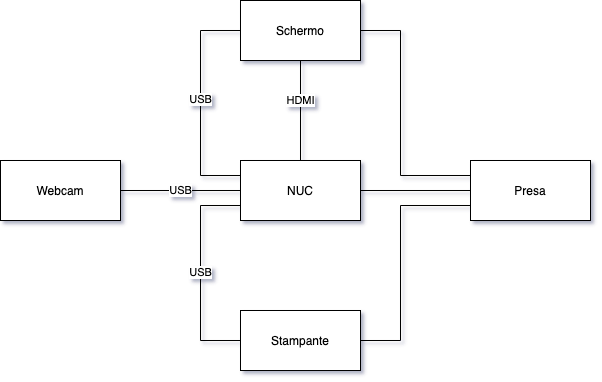
\includegraphics[width=0.7\textwidth]{img/cables_it.png}
                \caption{Schema dei vari collegamenti}
                \label{cables}
        \end{figure}
		
		
	\subsection{Avvio}
	
	\begin{enumerate}		
		\item Posizionare su 1 l'interruttore principale dello schermo, posizionato sul lato destro vicino al connettore di alimentazione
		\item Premere il pulsante di accensione del NUC
		\item Premere per qualche secondo il tasto \texttt{On} della stampante
		\item Quando si presenta la schermata di blocco di Windows, trascinare l'immagine verso l'alto e inserire la password \texttt{usi-warpme} con l'aiuto della tastiera a schermo
		\item Il software dovrebbe avviarsi automaticamente, mostrando un volto grigio. Qualora non fosse il caso, avviarlo toccando due volte l'icona \texttt{WarpMe} sul Desktop
	\end{enumerate}	
		
		
		
\section{Utilizzo}

	\subsection{Scattare una foto}

		Dalla schermata principale del software, toccare l'icona della fotocamera 
\includegraphics[width=1cm]{../src/resource/icons/camera.png} e posizionare il volto all'interno dell'area arancione.
		
		Una volta scattata la foto, deformarla a piacimento trascinando i punti arancioni sui bordi.        
	
	
	\subsection{Esportazione}
	
		Per stampare la foto, toccare l'icona di stampa 
\includegraphics[width=1cm]{../src/resource/icons/print.png}.
		
		Per ricevere la foto per email, toccare l'icona email 
\includegraphics[width=1cm]{../src/resource/icons/mail.png}, inserire il proprio indirizzo email e toccare 
\includegraphics[width=1cm]{../src/resource/icons/ok.png} per inviare.
		
	
	
\section{Spegnimento}
	
		\begin{enumerate}
			\item Premere brevemente il tasto di accensione del NUC
			\item Attendere e verificare che si sia spento completamente
			\item Posizionare su 0 l'interruttore dello schermo (lato destro)
			\item Spegnere la stampante premendo il tasto \texttt{On}
		\end{enumerate}
	
	
	
\section{Manutenzione}

	\subsection{Consumabili}
	
		Riferimento set carta e inchiostro: Canon KC-36IP. Può essere ordinato tramite il Copy Center all'USI (\url{https://www.desk.usi.ch/it/copy-center-campus-di-lugano}).
		

	\subsection{Carta stampante}		
		
		Per ricaricare il vassoio della carta, estrarlo dalla stampante e inserire la carta con la faccia lucida in alto e i bordi rettangolari in fondo.
		
		
	\subsection{Inchiostro stampante}
		
		Per sostituire la cartuccia, aprire lo sportello collocato sul lato destro della stampante, estrarre la cartuccia usata sollevando il gancio marrone e inserire delicatamente quella nuova, con l'etichetta verso l'alto. Smaltire in maniera appropriata le vecchie cartuccie.
		
		
		
\section{Codice sorgente}

	Il codice sorgente dell'applicazione, assieme alle istruzioni per compilarla, si trova qui: \url{https://github.com/USI-Showroom/WarpMe}.
		
	
\end{document}